\documentclass[letterpaper,11pt]{article}
\usepackage[brazil]{babel}
\usepackage[T1]{fontenc}
\usepackage{ae}
\usepackage[utf8]{inputenc}
\usepackage[dvipsnames]{color}
\usepackage{graphicx}
\usepackage{epsfig}
\usepackage{dci}
\usepackage{amssymb, amsmath, amsfonts}
\bibliographystyle{plain}
\topmargin		0 cm
\hoffset		-1 cm
\voffset		0 cm
\evensidemargin		0 cm
\oddsidemargin		0 cm
\setlength{\textwidth}{18 cm}
\setlength{\textheight}{21 cm}

\title{ As cr\^{o}nicas de Medrash }
\author{ Grupo 1A }
\date{ }

\begin{document}
\begin{center}
\begin{minipage}{2.4 cm}
\begin{center}

\includegraphics{logo.png}
\end{center}
\end{minipage}
\begin{minipage}{12 cm}
\begin{center}
\Large
UNIVERSIDADE ESTADUAL DE CAMPINAS \\
FACULDADE DE ENGENHARIA ELÉTRICA E DE COMPUTAÇÃO
\end{center}
\end{minipage}
\end{center}

\vspace{6 cm}
\begin{center}
{\bf \large PROPOSTA DO JOGO}
\vspace{0.5 cm}

Introdução ao Projeto de Jogos Digitais (IA369A) \\
Professor: José Mario De Martino \\
Primeiro Semestre de 2012
\end{center}
\vspace{3 cm}
\begin{flushright}
{\bf Grupo 1A} \\
Edgar Armeliato \\
Fernanda Leal \\
Harlei Miguel de Arruda Leite \\
Julián Prada Sanmiguel \\
Lauro Américo dos Santos \\
Maria Fernanda Rodriguez \\
Paúl Mejia \\
Rodrigo Mologni \\
Rodrigo Aparecido Morbach \\
Tiago Cinto \\
Thiago Cavalcante
\end{flushright}

\newpage
\tableofcontents
\newpage

{\bf Proposta do Jogo - Grupo 1A}

\section{Nome do Jogo}
As Crônicas de Medrash

\section{História}
Medrash é um homem primata, na casa dos 20 anos, que havia saído na noite anterior para caçar para sua tribo, Ari, como de costume.
Na manhã seguinte, ao voltar para casa, ele encontra sua tribo devastada após um ataque de uma tribo inimiga, Luskan, a mando de seu arqui-inimigo, Balasar. 
Ao percorrer o local, Medrash encontra um guerreiro ferido sobrevivente, o qual conta o ocorrido da noite passada: sua tribo havia sido atacada e seus amigos sequestrados para serem escravizados. Dentre os sequestrados estava Sora, sua mulher. Nosso herói precisa correr contra o tempo para salvar seus amigos e derrotar Balasar, fazendo alianças e lutando contra as mais diversas adversidades.

\section{Características Gerais}
\begin{itemize}
\item {\bf Estilo} Ação/Aventura
\item {\bf Perspectiva} Câmera atrás do personagem, fixa em relação a ele.
\item {\bf Modo} Monojogador.
\item {\bf Número de Fases} 3 fases.
\item {\bf Linha do Tempo} Pré-Histórico
\item {\bf Objetivo do Jogo} Resgatar sua tribo, incluindo Sora, de Balasar e sua tribo Luskan, que tentam escravizá-los.
\item {\bf Referências} Crash Bandicoot, Super Mario 64, Zelda, Pitfall 3D.
\item {\bf HUD} Vida, Temperatura, Alimentação.
\end{itemize}

\section{Personagens}

\subsection{Medrash - Personagem Principal}
Homem pré-histórico, na casa dos 20 anos.

\subsection{Sora - Esposa}
Mulher de Medrash, na casa dos 18 anos. Foi raptada por Balasar.

\subsection{Balasar - Arqui-inimigo}
Chefe da tribo Luskan, na casa dos 25 anos. Pretende escravizar as outras tribos.

\subsection{Gardain - Primeiro Guerreiro}
Amigo de Medrash, na casa dos 20 anos. Encontrado machucado por Medrash. É o personagem responsável por avisar Medrash do ataque inimigo.

\subsection{Rangrim - Líder da tribo Mara-kai}
Líder da tribo Mara-kai, na casa dos 35 anos.
Envia Medrash à tribo Akanul por um atalho.

\subsection{Animais Selvagens}
Lobos, tigres, jacarés, e outros animais que atacam Medrash.

\subsection{Integrantes da tribo Luskan}
Inimigos genéricos.

\section{Descrição das Fases}
  \subsection{Tutorial}
Um tutorial com o jogador aprendendo a usar os comandos básicos, fazer fogo e obter alimento.

  \subsection{Fase 1}
{\it CINEMATICS: Medrash volta para sua tribo, Ari, e encontra Gardain machucado e o resto do seu grupo desaparecido.
Gardain o informa que seu grupo foi atacado pela tribo Luskan, e que pessoas de seu grupo foram sequestrados, incluindo Sora, sua mulher.}

Medrash inicia a fase com um porrete e deverá percorrer uma trilha deixada pelo inimigo. No percurso, ele enfrenta vários obstáculos e animais selvagens que servirão de alimento.
No caminho, ele poderá encontrar um guerreiro morto e pegar a sua lança. No fim da trilha existe um tigre fechando o caminho. Para prosseguir, Medrash deverá matá-lo. Ao derrotá-lo, o dia estará chegando ao fim.

  \subsection{Fase 2}
{\it CINEMATICS: Medrash está chegando na tribo Mara-kai, e vê eles sendo atacados pela tribo Luskan.}

Ao chegar em Mara-kai, Medrash é informado por Rangrim que a tribo de Luskan se dirige à tribo aliada de Akanul. Rangrim pede que Medrash dirija-se ao local e avise-os, tomando um atalho pelas montanhas à noite. O percurso é cheio de perigos, e Medrash deve usar o fogo para afastar os animais selvagens. Ele também deve usar o fogo para se aquecer, e deverá cuidar para mantê-lo aceso.
Medrash chega na tribo Mara-kai a tempo de avisá-los. O ataque de Luskan acontece logo em seguida e eles conseguem rechaça-lo.

  \subsection{Fase 3} 
{\it CINEMATICS: As tribos Akanul e Mara-kai se aliam para atacar Luskan.}

Medrash enfrenta soldados para libertar as pessoas escravizadas das tribos aliadas. Após libertar alguns grupos, ele é informado do local onde Balasar está com sua amada Sora. Medrash irá resgatá-la e, para isso, terá que derrotar seu arqui-inimigo Balasar, em uma disputa corpo-a-corpo.

 \subsection{Epílogo}
 {\it CINEMATICS: Medrash salva Sora, e liberta o restante dos escravos. Gardain já está curado e todos vivem felizes para sempre.}

\section{Jogabilidade}
O personagem poderá se mover livremente pelo cenário, em todas as direções disponíveis no mapa.

O jogador irá controlar o personagem principal com as teclas direcionais do teclado (cima, baixo, esquerda e direita). 
Para o restante das açôes, as teclas `a', `s', `d' e `espaço' serão utilizadas para controlar o ataque, ações diversas, defesa e para pular, respectivamente.

\section{Características do Cenário}

\subsection{Cenário 1}
 O cenário inicial exibe a tribo destruída de Medrash. Utilizado no início da fase 1.

\subsection{Cenário 2}
 O próximo cenário é constituído por animais selvagens e este espaço permite que o personagem desloque-se soubre um ambiente ampla que se afunila com a proximidade ao final. Utilizado na fase 1.

\subsection{Cenário 3}
 Este cenário é similar ao primeiro, porém com efeitos que refletem a um ataque recente, como fogo e fumaça. Utilizado no início da fase 2.

\subsection{Cenário 4}
 Este cenário é formado por um ambiente escuro e com neve, similar ao cume de uma montanha. Utilizado na fase 2.

\subsection{Cenário 5}
 Uma grande tribo rodeada de montanhas. Utilizado no final da fase 2.

\subsection{Cenário 6}
 Um ambiente árido amplo no qual estão os grupos aprisionados. Utilizado na fase 3.

\subsection{Cenário 7}
 Cenário em aberto. Utilizado no confronto final entre Medrash e Balasar.

\section{Características da IA}
 Todos os inimigos básicos seguirão a Máquina de Estados a seguir:
 \begin{center}
  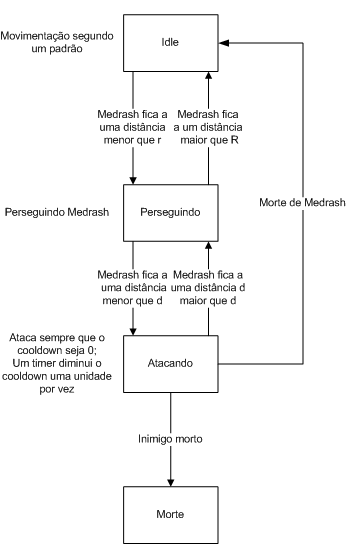
\includegraphics[scale=1.2]{ia_simples.png}
 \end{center}
 As máquinas de estados específicas serão construídas em cima desse modelo.

\subsection{Animais Selvagens}
 Acreditamos que os animais selvagens seguirão essa máquina de estados com pequenas modificações de comportamento.

\subsection{Inimigos Comuns}
 Os inimigos devem incluir um estado para fugir ou defender.

\subsection{Chefes - Inimigos Especiais}
 A Inteligência Artificial dos chefes será variada podendo incluir defesa e ataques especiais.

\section{Plataforma de Desenvolvimento}
 Discutimos sobre a utilização de três plataformas:
 \begin{itemize}
  \item XNA
  \item UDK
  \item Unity
 \end{itemize}
 A plataforma XNA tem nível baixo para nossos requerimentos. 
A plataforma UDK não se mostrou estável nos testes, além de ser muito pesada. 
A plataforma Unity foi a preferida, por facilitar bastante o desenvolvimento.

A plataforma Unity permite criar facilmente os controles de movimentação, o terreno e a física. Podemos escrever scripts em \verb+C#+, \verb+Javascript+ e \verb+Boo+.

\end{document}

